\chapter{Applications}

We investigate numerical methods for equations describing real life problems.

\section{The Navier Stokes equation}

The Navier Stokes equation describe the flow of a fluid (such as water or air).
The incompressible Navier Stokes equation models incompressible fluids (such as water).
The stationary N.-St. equation models a solution in steady state (no change in time).

The field variables are the fluid velocity $u = (u_x, u_y, u_z)$, and the pressure $p$. 
Conservation of momentum is
$$
-\nu \Delta u + \rho (u \cdot \nabla) u - \nabla p = f
$$
The first term describes friction of the fluid ($\nu$ is called viscosity).
The second one arises from conservation of momentum of moving particles. 
It is called the convective term ($\rho$ is the density).
The source term $f$ models forces, mainly gravity.
The incompressibility of the fluid is described by
$$
\opdiv \, u = 0.
$$
Different types of boundary conditions onto $u$ and $p$ are possible.

\bigskip

The Navier Stokes equation is nonlinear. In general, no unique solution is 
guaranteed. 
The common approach to find a solution is the so called Oseen iteration: Given $u^k$,
find the next iterate $(u^{k+1},p^{k+1})$ by solving
\begin{eqnarray*}
-\nu \Delta u^{k+1} + \rho (u^k \cdot \nabla) u^{k+1} - \nabla p^{k+1} & = & f \\
\opdiv \, u^{k+1} & = & 0.
\end{eqnarray*}

Under reasonable conditions, this Oseen equation is uniquely solvable. Since $u^k$
is the solution of the old step, it satisfies $\opdiv \,  u^k = 0$. Furthermore, we
assume that the velocity $u^k$ is bounded in $L_\infty$-norm.

\bigskip
From now on, we continue to investigate the Oseen equation. Given a vector-field
$w = (w_x, w_y, w_z) \in [L_\infty]^3$ such that $\opdiv \, w = 0$. Find $u$ and $p$ 
such that
\begin{eqnarray*}
-\Delta u + (w \cdot \nabla) u - \nabla p & = & f \\
\opdiv \, u & = & 0.
\end{eqnarray*}
We have removed the viscosity by rescaling the equation. The factor $\rho/\nu$ is
incorporated into the vector-field $w$.


\bigskip

As usual, we go over to the weak formulation: Find $u \in V = [H^1]^3$ and $p \in Q = L_2$
such that
\begin{equation} \label{equ_weakoseen}
\begin{array}{ccccll}
\int \{ \nabla u \, \nabla v + (w\cdot \nabla) u \, v \} \, dx & + & \int \opdiv \, v \, p \, dx & = & \int f v \, dx \quad  & \forall \, v \in V \\
\int \opdiv u \, q \, dx & & & = & 0  & \forall \, q \in Q.
\end{array}
\end{equation}

This variational problem is a mixed formulation. It satisfies the conditions of Brezzi:
The bilinear forms are
\begin{eqnarray*}
a(u,v) & = & \int \{ \nabla u \nabla v + (w\cdot \nabla) u v \} \, dx, \\
b(u,q) & = & \int \opdiv \, u \, q \, dx.
\end{eqnarray*}

Both forms are continuous. The form $a(.,.)$ is non-symmetric.
In $a(.,.)$, the $x$, $y$, and $z$ components of $u$ and $v$ are independent. 
To investigate $a(.,.)$, it is enough to consider scalar bilinear-forms. 
We define the inflow and outflow boundaries
\begin{eqnarray*}
\Gamma_i & = & \{ x \in \partial \Omega : w \cdot n < 0 \}, \\
\Gamma_o & = & \{ x \in \partial \Omega : w \cdot n \geq 0 \}.
\end{eqnarray*}
If we pose Dirichlet boundary conditions on $\Gamma_i$, then $a(.,.)$ is 
coercive (see example~\ref{example_diffconv}, and exercises). 
The ratio of the continuity bound and the coercivity bound depends on the
norm of the convection $w$. With increasing $w$, the problem is getting worse.


The form $b(.,.)$ satisfies the LBB condition:
$$
\sup_{u \in [H_{0,D}^1]^3} \frac{ \int \opdiv u \, q \, dx } { \| u \|_{H^1} } \geqc \| q \|_{L_2} \qquad \forall \, q \in L_2.
$$
In the case of (partial) Dirichlet boundary conditions ($H_{0,D}^1 = \{ u : u = 0 \; \mbox{on} \; \Gamma_D \}$), this condition is very nontrivial to prove. If there are only Dirichlet b.c.,
one has to use $Q = L_2^0 = \{ q : \int_\Omega q \, dx = 0 \}$.

Under these conditions, Brezzi's theorem proves a unique solution of the Oseen equation.

\bigskip

\subsubsection{Finite elements for Navier-Stokes equation}

We want to approximate the Oseen equation by a Galerkin method: Find $u_h \in V_h$ and
$p_h \in Q_h$ such that
\begin{equation} \label{equ_weakoseenfem}
\begin{array}{ccccll}
\int \{ \nabla u_h \, \nabla v_h + (w\cdot \nabla) u_h \, v_h \} \, dx & + & \int \opdiv \, v_h \, p_h \, dx & = & \int f v_h \, dx \quad  & \forall \, v_h \in V_h \\
\int \opdiv u_h \, q_h \, dx & & & = & 0  & \forall \, q_h \in Q.
\end{array}
\end{equation}

To obtain convergence $u_h \rightarrow u$ and $p_h \rightarrow p$, it is important
to choose proper approximation spaces $V_h$ and $Q_h$. Using the simplest elements,
namely continuous and piece-wise linear elements for $V_h \subset [H^1]^3$, and piece-wise 
constants
for $Q_h \subset L_2$ does not work. The discrete LBB condition is not fulfilled:
In 2D, there are asymptotically twice as many triangles than vertices, i.e.,
dim $V_h \approx$ dim $Q_h$, and $\int \opdiv u_h \, q_h \,dx = 0 \; \forall \, q_h \in Q_h$ implies $u_h \approx 0$.

\bigskip

The simplest spaces which lead to convergence are the non-conforming $P_1$ element 
for the velocities, and piece-wise constant elements for the pressure. The arguments are
\begin{itemize}
\item
There are unknowns on the edges to construct a Fortin operator satisfying
$$
\int_e u \cdot n \, ds = \int_e  (I_h u) \cdot n \, ds,
$$
and thus proving the discrete LBB condition.
\item
The error due to the non-conforming space $V_h \not\subset V$ is of the same
order as the approximation error (see Section~\ref{sec_nonconforming}).
\end{itemize}

% \documentclass[12pt]{article}
% \usepackage{amsmath,amsthm,amssymb,a4wide}
% \usepackage[german,english]{babel}
% \usepackage{epsfig}
% \usepackage{latexsym}
% \usepackage{amssymb}
% % \usepackage{theorem}
% \usepackage{amsthm}
% % \usepackage{showkeys}

% \newcommand{\setR}{ {\mathbb R} }
% \newcommand{\setN}{ {\mathbb N} }
% \newcommand{\setZ}{ {\mathbb Z} }
% \newcommand{\eps}{\varepsilon}

% \newcommand{\beq}{\begin{equation}}
% \newcommand{\eeq}{\end{equation}}

% \newcommand{\opdiv}{\operatorname{div}}
% \newcommand{\opcurl}{\operatorname{curl}}
% \newcommand{\opdet}{\operatorname{det}}
% \newcommand{\optr}{\operatorname{tr}}
% \newcommand{\optrn}{\operatorname{tr}_n}
% \newcommand{\sfrac}[2]{ { \textstyle \frac{#1}{#2} } }

% \newcommand{\Zh}{\mathrm{Z}_h}
% \newcommand{\Ih}{\mathrm{I}_l}

% \newcommand{\leqc}{\preceq} 
% \newcommand{\geqc}{\succeq} 
% \newcommand{\eqc}{\simeq} 
% \newcommand{\ul}{\underline}

% \newtheorem{theorem}{Theorem}
% \newtheorem{definition}[theorem]{Definition}
% \newtheorem{lemma}[theorem]{Lemma}
% \newtheorem{remark}[theorem]{Remark}
% \newtheorem{example}[theorem]{Example}

% %
% %
% \setlength{\unitlength}{1cm}
% \sloppy 
% %

% \title{Proving LBB for the Stokes Equation}
% \author{Joachim Sch\"oberl}

% \begin{document}
% \maketitle
% \centerline{(supplement to lecture notes Chapter 8.1) } 

\subsection{Proving LBB for the Stokes Equation}
\subsubsection{Stability of the continuous equation}

We consider Stokes equation: find $u \in [H_0^1]^d$ and $p \in L_2^0$ such that
\begin{equation}
\begin{array}{ccccll}
\int \nabla u \cdot \nabla v & + & \int \opdiv v \, p & = & \int f v \quad & \forall \, v \in [H_0^1]^d \\[0.5em]
\int \opdiv u \, q && & = & 0 & \forall \, q \in L_2^0.
\end{array}
\end{equation}
Solvability follows from Brezzi's theorem. The only non-trivial part is the LBB condition:
$$
\sup_{v \in [H_0^1]^d} \frac { \int \opdiv v \, p}  { \| v \|_{H^1}} \geq \beta \| p \|_{L_2}
\qquad \forall \, p \in L_2^0
$$ 
We sketch two different proofs: 

{\em Proof 1: } The LBB condition becomes simple if we skip the Dirichlet conditions:
$$
\sup_{v \in [H^1]^d} \frac { \int \opdiv v \, p}  { \| v \|_{H^1}} \geq \beta \| p \|_{L_2}
\forall \, p \in L_2
$$
Take $p \in L_2(\Omega)$, extend it by $0$ to $L_2 (\setR^d)$. Now compute a right-inverse of $\opdiv$ via Fourier transform:
\begin{eqnarray*}
\hat p(\xi) & = & {\mathcal F} (p) \\
\hat u(\xi) & = & \frac{-i\xi}{|\xi|^2} \hat p(\xi) \\
u(x) & = & {\mathcal F}^{-1} (\hat u ) \\
\end{eqnarray*}
Since $\opdiv u = p$ translates to $i \xi \cdot \hat u = \hat p$, we
found a right-inverse to the divergence. Furthermore, $| u
|_{H^1(\Omega)} = \| i \xi \hat u\|_{L_2} \leqc \| \hat p \|_{L_2} =
\| p \|_{L_2}$. We restrict this $u$ to $\Omega$. 
The $L_2$-part of $\| u \|_{H^1}$ follows from the
Poincare inequality after subtracting the mean value. 

The technical part is to ensure Dirichlet - boundary conditions. One can build an extension operator ${\mathcal E}$ from $L_2(\setR^d \setminus \Omega)$ onto $\setR^d$, which commutes with the $\opdiv$-operator: $\opdiv {\mathcal E} u = {\mathcal E}^p \opdiv u$, and sets
$$
u_{final} := u - {\mathcal E} u
$$
This $u$ satisfies $u = 0$ on $\partial \Omega$. Since $\opdiv u = p = 0$ outside of $\Omega$, the correction did not change the divergence inside $\Omega$.

{\em Proof 2: } Directly construct a right-inverse for the $\opdiv$-operator via integration. We assume that $\Omega$ is star-shaped w.r.t. $\omega$, and $a\in \omega$. Extend $p$ by $0$ to $L_2(\setR^d)$:
$$
u_a(x) := -(x-a) \int_1^\infty  t^{d-1} p(a + t(x-a)) \, dt\qquad x
\neq a
$$
and $u_a(a) = 0$.
If $\int_\Omega p = 0$, then $\opdiv u_a = p$. Furthermore, $u = 0$ outside $\Omega$.
Next, we average over star-points in $\omega$:
$$
u := \frac{1}{|\omega|}  \int_\omega u_a \, da
$$
There is still $\opdiv u = p$. Now, one can show that $\| u \|_{H^1} \leqc \| p \|_{L_2}$

\subsection{Discrete LBB}

Now, we turn to the discrete system posed on $V_h \subset V$ and $Q_h \subset Q$. 
The discrete LBB condition follows from the continuous one by
construction of a Fortin operator (Lemma~99).

\subsubsection{Elements with discontinuous pressure}
The simplest pair is the non-conforming $P^1$ element, and constant pressure:
$$
V_h  = P^{1,nc}, \qquad Q_h = P^{0,dc}
$$
We have to extend the $V$-norm and forms by the sum over element-wise norms and forms.
The Fortin-operator $I_F : V \rightarrow V_h$ is defined via
$$
\int_E I_F u = \int_E u \quad \forall \, \text{edges } E
$$
It is continuous from $H^1$ to broken $H^1$ (via mapping), and satisfies
$$
\int_T \opdiv (I_F u) = \int_{\partial T} (I_F u) \cdot n = \int_{\partial T} u \cdot n = \int_T \opdiv u,
$$
and thus
$$
b_h(I_F u, q_h) = b(u, q_h) \qquad \forall \, q_h \in Q_h
$$
The error estimate follows similar as in the second Lemma by Strang:
\begin{eqnarray*}
\lefteqn{\| u - u_h\|_{H^1,nc} + \| p - p_h \|_{L_2}} \\
& \leqc &\inf_{v_h, q_h} \| u - v_h \|_{H^1,nc} + \| p - q_h\|_{L_2} 
+ \sup_{w_h} \frac{ \sum_T \int \nabla u \nabla w_h   + p \opdiv w_h - f w_h} {\| w_h \|_{H^1,nc} } \\
& \leqc & c h \, (  \| u \|_{H^2} + \| p \|_{H^1} )
\end{eqnarray*}
This convergence rate $O(h)$ is considered to be optimal for these elements.

Next we consider
$$
V_h = P^2 \qquad Q_h = P^{0,dc}
$$
We would like to define the Fortin operator similar as before:
$$
\begin{array}{rcll}
I_F u(V) & = & u(V)  \quad & \forall \, \text{vertices } V \\[0.5em]
\int_E I_F u & = & \int_E u \quad & \forall \, \text{edges } E
\end{array}
$$
But, the vertex evaluation is not allowed in $H^1$. We proceed now in two steps: First approximate $u$ in the finite element space via a Cl\'ement operator $\Pi_h$:
$$
u_h^1 := \Pi_h u,
$$
and modify this $u_h^1$ via a correction term:
$$
u_h := I_F u := u_h^1 + I_F^2 (u - u_h^1)
$$
The correction operator $I_F^2$ is defined as
$$
\begin{array}{rcll}
I_F^2 u(V) & = & 0  \quad & \forall \, \text{vertices } V, \\[0.5em]
\int_E I_F^2 u & = & \int_E u \quad & \forall \, \text{edges } E.
\end{array}
$$
It preserves edge-integrals and thus satisfies $b(u - I_F^2 u, q_h) =
0 \; \forall \, u \; \forall \, q_h$. Furthermore, it is continuous with respect to
$$
\| I_F^2 u \|_{H^1} \leqc \| u \|_{H^1} + h^{-1} \| u \|_{L_2}
$$
Thus, the combined operator $I_F$ is continuous:
\begin{eqnarray*}
\| I_F u \|_{H^1} & \leqc & \| \Pi_h u \|_{H^1} + \| I_F^2 (u-\Pi_h u) \|_{H1} \\
    & \leqc & \| u \|_{H^1} + \| u - \Pi_h u\|_{H^1} + h^{-1 } \| u - \Pi_h u \|_{L_2} \\
   & \leqc & \|  u \|_{H^1}
\end{eqnarray*}
It also satisfies the constraints:
$$
b(u - I_F u, q_h) = b(u - \Pi_h u - I_F^2 (u - \Pi_h u), q_h) = b( (Id - I_F^2)(u - \Pi_h u), q_h) = 0 
$$
Error estimates are
$$
\| u - u_h \|_{H^1} + \| p  - p_h \|_{L_2} \leqc \inf_{v_h, q_h} \| u - v_h \|_{H^1} + \| p - q_h \|_{L_2} 
= O(h)
$$
Although we approximate $u_h$ with $P^2$-elements, the bad
approximation of $p$ leads to first order convergence, only. This
element is considered to be sub-optimal.

A solution is the the pairing
$$
V_h = P^{2+} \qquad Q_h = P^{1, nc},
$$
where $P^{2+}$ is the second order space enriched with cubic bubbles:
$$
P^{2+}({\mathcal T}) = \{ v_h \in H^1 : v_{h|T} \in P^3(T), v_{h|E} \in P^2(E) \}
$$
It leads to second order convergence. Since the costs of a method depend mainly on the coupling dofs, the price for the additional bubble is low.

\subsubsection{Elements with continuous pressure}
Although the pressure $p$ is only in $L_2$, we may approximate it with
continuous elements. The so called mini-element is
$$
V_h = P^{1+} \qquad Q_h = P^{1,cont},
$$
where $P^{1+}$ is $P^1$ enriched by the cubic bubble. The continuous
pressure allows integration by parts:
$$
\int \opdiv u \, q_h = - \int u \nabla q_h
$$
The gradient of $q_h$ is element-wise constant. We thus construct a
Fortin-operator
preserving element-wise mean values. Again, we use the Cl\'ement operator
and a  correction operator:
$$
u_h := I_F u = \Pi_h u + I_F^2 (u - \Pi_h u)
$$
The correction is now defined as
$$
\begin{array}{rcll}
I_F^2 u & = & 0  \quad & \text{on} \cup E  \\
\int_T I_F^2 u & = & \int_T u \quad & \forall \, \text{elements } T.
\end{array}
$$
It satisfies $b(u - I_F^2 u, q_h) = 0 \qquad \forall \, u \, \forall
\, q_h$, and, as above:
$$
\| I_F^2 u \|_{H^1} \leqc \| u \|_{H^1} + h^{-1} \| u \|_{L_2}
$$
Thus, the combined operator is a Fortin operator.
This method is $O(h)$ convergent.
\medskip

Another (essentially) stable pair is $P^2 \times P^{1,cont}$ (the
popular Taylor Hood element). Its analysis is more involved. 
It requires the additional assumption that no two edge of one element are
on the domain boundary. Its convergence rate is $O(h^2)$.
% \end{document}

\section{Elasticity}

We start with a one-dimensional model. Take a beam which is loaded by a force density $f$
in longitudinal ($x$) direction. We are interested in the displacement $u(x)$ in $x$
direction.

The variables are
\begin{itemize}
\item The {\em strain $\eps$}: It describes the elongation. Take two points $x$ and $y$ on 
the beam. After deformation, their distance is $y+u(y) - (x+u(x))$. The relative elongation 
of the beam is
$$
\frac{ \left\{ y+u(y) - (x+u(x)) \right\}  - (y-x) }{y-x} = \frac{u(y)-u(x)}{y-x}.
$$
In the limit $y \rightarrow x$, this is $u^\prime$. We define the strain $\eps$ as
$$
\eps = u^\prime.
$$
\item The {\em stress $\sigma$}: It describes internal forces. If we cut the piece $(x,y)$ 
out of the beam, we have to apply forces at $x$ and $y$ to keep that piece in equilibrium.
This force is called stress $\sigma$. Equilibrium is
$$
\sigma(y) - \sigma(x) + \int_x^y f(s) \, ds = 0,
$$
or 
$$
\sigma^\prime = -f
$$
\end{itemize}
Hook's law postulates a linear relation between the strain and the stress:
$$
\sigma = E \eps.
$$
Combining the three equations
$$
\eps = u^\prime \qquad \sigma = E \eps \qquad \sigma^\prime = -f
$$
leads to the second order equation for the displacement $u$:
$$
-(E u^\prime)^\prime = f.
$$

Boundary conditions are
\begin{itemize}
\item Dirichlet b.c.: Prescribe the displacement at the boundary
\item Neumann b.c: Prescibe the stress at the boundary
\end{itemize}

\subsubsection{Elasticity in more dimensions}
We want to compute the deformation of the body $\Omega \subset \setR^d$.
\begin{itemize}
\item
The body is loaded with a volume force density $f : \Omega \rightarrow \setR^d$.
\item
The displacement is described by a the vector-valued function
$$
u : \Omega \rightarrow \setR^d.
$$
\item
The strain $\eps$ becomes a symmetric tensor in $\setR^{d\times d}$. The elongation in
the direction of the unit-vector $n$ is
$$
n^T \eps n.
$$
The (linearized!) relation between the displacement $u$ and the strain is now
$$
\eps_{ij} = \frac{1}{2} \left\{ \frac{\partial u_i}{\partial x_j} + \frac{\partial u_j}{\partial x_i} \right\},
$$
or, in compact form
$$
\eps = \eps(u) = \frac{1}{2} \left\{ \nabla u + (\nabla u)^T \right\}.
$$
If the displacement is a pure translation (u = const), then the strain vanishes.
Also, if the displacement is a linearized (!) rotation, 
(in two dimensions $u = (u_x,u_y) = (y,-x)$, the strain vanishes. 
We call these deformations the rigid body motions:
\begin{eqnarray*}
R^{2D} & = & \left\{ \left( a_1 \atop a_2 \right) + b \left( y \atop -x \right) : a_1, a_2, b \in \setR \right\} \\[0.5em]
R^{3D} & = & \left\{ a + b \times x : a, b \in \setR^3 \right\}
\end{eqnarray*}
\item 
The stress becomes a tensor $\sigma \in \setR^{d\times d}$. Consider the part $V \subset \Omega$. To keep $V$ in equilibrium, on has to apply the surface force density $\sigma n$ at $\partial V$:
$$
\int_{\partial V} \sigma n \, ds + \int_V f \, dx = 0.
$$
Apply Gauss theorem to obtain the differential form
$$
\opdiv \, \sigma = -f.
$$
The $\opdiv$-operator is applied for each row of $\sigma$. A further hypothesis, 
equilibrium of angular momentum, implies that $\sigma$ is symmetric.
\item
Hook's law is now a relation between two second order tensors:
$$
\sigma_{ij} = \sum_{kl} D_{ijkl} \eps_{kl},
$$
in short
$$
\sigma = D \eps,
$$
where $D$ is a fourth order tensor. For an isotropic material (same properties in all 
directions), the matrial law has the special structure
$$
\sigma = 2 \mu \, \eps + \lambda \, \optr \{ \eps \} \, I.
$$
The two parameters $\mu$ and $\lambda$ are called Lam\'e's parameters. The trace $\optr$
is defined as $\optr \{ \eps \} = \sum_{i=1}^d \eps_{ii}$.
\end{itemize}

Collecting the equations
$$
\eps = \eps(u) \qquad \sigma = D \eps \qquad \opdiv \, \sigma = -f
$$
leads to
$$
-\opdiv \, D \, \eps(u) = f.
$$
\bigskip

Multiplication with test-functions $v : \Omega \rightarrow \setR^d$, and integrating by parts 
leads to
$$
\int_\Omega D \, \eps(u) : \nabla v \, dx = \int f \cdot v \, dx \qquad \forall \, v 
$$
The operator '$:$' is the inner product for matrices, $A:B = \sum_{ij} A_{ij} B_{ij}$.
Next, we use that $\sigma = D \eps(u)$ is symmetric. Thus, $\sigma : \nabla v = \sigma : (\nabla v)^T = \sigma : \frac{1}{2} \{ \nabla v + (\nabla v)^T \}$. 

\bigskip

The equations of elasticity in weak form read as: Find $u \in V = [H_{0,D}^1(\Omega)]^d$
such that
$$
\int_\Omega D \eps(u) : \eps(v) \, dx = \int_\Omega f \cdot v \, dx \qquad \forall \, v \in V.
$$

Displacement (Dirichlet) boundary conditions ($u = u_D$ at $\Gamma_D$) are essential b.c., 
and are put into the
space~$V$. Neumann boundary conditions (natural b.c.) model surface forces $sigma n = g$,
and lead to the additional term $\int_{\Gamma_N} g \cdot v \, ds$ on the right hand side.

\bigskip

The bilinear-form in the case of an isotropic material reads as
$$
\int 2 \mu \, \eps(u) : \eps(v)  + \lambda \, \opdiv \, u \; \opdiv \, v \, dx.
$$


We assume a positive definite material law 
$$
D \eps : \eps \geqc \eps : \eps \qquad \forall \, \mbox{symmetric} \; \eps \in \setR^{d\times d}
$$
\begin{theorem} Assume that the Dirichlet boundary $\Gamma_D$ has positive measure.
Then the equations of elasticity are well posed in $[H^1]^d$.
\end{theorem}
{\em Proof:} Continuity of the bilinear-form and the linear-form are clear.
Ellipticity of the bilinear-form follows from the positive definite matrial law, and 
the (non-trivial) Korn inequality
$$
\int_\Omega \eps(u) : \eps (v) \, dx \geqc \| u \|_{H^1(\Omega)}^2 \qquad \forall \, u \in [H_{0,D}^1]^d
$$
The Lax-Milgram theorem proves a unique solution $u$.
\hfill $\Box$

\bigskip

The discretization of the elasticity problem is straight forward. Take a finite dimensional
sub-space $V_h \subset V$, and perform Galerkin projection. One may use the 'standard'
nodal finite elements for each component. 

\subsubsection{Structural mechanics}
Many engineering applications involve thin structures (walls of a building, body of a car, ...).
On thin structures, the standard approach has a problem: One observed that the simulation
results get worse as the thickness decreases. The explanation is that the constant in 
Korn's inequality gets small for thin structures. To understand and overcome this problem,
we go over to beam, plate and shell models. 

\bigskip

We consider a thin ($t \ll 1$) two-dimensional body
$$
\Omega = I \times (-t/2, t/2) \qquad \mbox{with} \qquad I = (0,1)
$$
The goal is to derive a system of one-dimensional equations to describe the two-dimensional
deformation. This we obtain by a semi-discretization. Define
$$
\widetilde V_M = \left\{ \left(u_x(x,y) \atop u_y(x,y) \right) \in V :
 u_x(x,y) = \sum_{i=0}^{M_x} u_x^i(x) y^i , \; u_y(x,y) = \sum_{i=0}^{M_y} u_y^i(x) y^i \right\}.
$$
This function space on $\Omega \subset \setR^2$ is isomorph to a one-dimensional 
function space with values in $\setR^{M_x+M_y+2}$. We perform semi-discretization 
by searching for
$\tilde u \in \widetilde V_M$ such that
$$
A(\tilde u, \tilde v) = f(\tilde v) \qquad \forall \, \tilde v \in \widetilde V_M.
$$
As $M_x, M_y \rightarrow \infty$, $\widetilde V_M \rightarrow V$, and 
we obtain convergence $\tilde u \rightarrow u$. 

\bigskip
The lowest order (qualitative) good approximating semi-discrete space is to set
$M_x = 1$ and $M_y = 0$. This is
$$
\widetilde V = \left\{ \left( U(x) - \beta(x) y  \atop w(x) \right) \right\}
$$

Evaluating the bilinear-form (of an isotropic material) leads to 
\begin{eqnarray*}
  A\left( \left( U - y \beta \atop w \right), \left( \tilde U - y \tilde \beta \atop \tilde w \right) \right) & = & 
  (2 \mu + \lambda) t \int_0^1 U^\prime \tilde U^\prime \, dx + \\
&&  (2 \mu + \lambda) \frac{t^3}{12} \int_0^1 \beta^\prime \tilde \beta^\prime + 
  2 \mu \frac{t}{2} \int_0^1 (w^\prime - \beta) (\tilde w^\prime - \tilde \beta) \, dx
\end{eqnarray*}


The meaning of the three functions is as follows. The function $U(x)$ is the average 
(over the cross section) longitudinal displacement, $w(x)$ is the vertical displacement.
The function $\beta$ is the linearized rotation of the normal vector.

\bigskip

We assume that the load $f(x,y)$ does not depend on $y$. Then, the linear form is
$$
f \left( \tilde U-y \tilde  \beta \atop \tilde w \right) = 
t \int_0^1 f_x \tilde U \, dx + t \int_0^1 f_y \tilde w \, dx
$$

The semi-discretization in this space leads to two decoupled problems. The first one
describes the longitudinal displacement: Find $U \in H^1(I)$ such that
$$
(2 \mu + \lambda) t \, \int_0^1 U^\prime \tilde U^\prime \, dx = 
t \int_0^1 f_x \tilde U^\prime \, dx \qquad \forall \, U^\prime \in H^1(I).
$$
The small thickness parameter $t$ cancels out. It is a simple second order problem
for the longitudinal displacement.

\medskip

The second problems involves the 1D functions $w$ and $\beta$: Find $(w,\beta) \in V = ?$
such that
$$
(2\mu+\lambda) \frac{t^3}{12} \int_0^1 \beta^\prime \tilde \beta^\prime \, dx + \mu t \int_0^1 (w^\prime - \beta) (\tilde w^\prime - \tilde \beta) \, dx = t \int_0^1 f_y \tilde w \, dx
\qquad \forall \, (\tilde w, \tilde \beta) \in V
$$
The first term models bending. The derivative of the rotation $\beta$ is (approximative)
the curvature of the deformed beam. The second one is called the shear term: For thin
beams, the angle $\beta \approx \tan \beta$ is approximatively $w^\prime$. This term
measures the difference $w^\prime - \beta$. 
This second problem is called the Timoshenko beam model. 


\bigskip

For simplification, we skip the parameters $\mu$ and $\lambda$, and the constants. 
We rescale the equation by dividing by $t^3$: Find $(w,\beta)$ such that
\begin{equation} \label{equ_timo}
\int \beta^\prime \tilde \beta^\prime \, dx + \frac{1}{t^2} \int (w^\prime - \beta) (\tilde w^\prime - \tilde \beta) \, dx = \int t^{-2} f \tilde w \, dx.
\end{equation}

This scaling in $t$ is natural. With $t \rightarrow 0$, and a force density $f \sim t^2$,
the deformation converges to a limit. We define the scaled force density
$$
\tilde f = t^{-2} f
$$

In principle, this is a well posed problem in $[H^1]^2$:

\begin{lemma} Assume boundary conditions $w(0) = \beta(0) = 0$. The 
bilinear-form $A((w,\beta), (\tilde w, \tilde \beta))$ of (\ref{equ_timo}) is 
continuous
$$
A( (w,\beta), (\tilde w, \tilde \beta)) \leqc t^{-2} 
( \| w \|_{H^1} + \| \beta \|_{H^1} ) ( \| \tilde w \|_{H^1} + \| \tilde \beta \|_{H^1} )
$$
and coercive
$$
A ( (w, \beta), (w, \beta) ) \geq \| w \|_{H^1}^2 + \| \beta \|_{H^1}^2
$$
\end{lemma}
{\em Proof: } ...

As the thickness $t$ becomes small, the ratio of the continuity and coercivity 
bounds becomes large ! This ratio occurs in the error estimates, and indicates 
problems. Really, numerical computations show bad convergence for small thickness $t$.

The large coefficient in front of the term $\int (w^\prime - \beta) (\tilde w^\prime - \tilde \beta)$ forces the difference $w^\prime - \beta$ to be small. If we use piece-wise linear
finite elements for $w$ and $\beta$, then $w_h^\prime$ is a piece-wise constant function,
and $\beta_h$ is continuous. If $w_h^\prime - \beta_h \approx 0$, then $\beta_h$ must
be a constant function !

\bigskip

The idea is to weaken the term with the large coefficient. We plug in the 
projection~$P^0$ into piece-wise constant functions: Find $(w_h, \beta_h)$ such that
\begin{equation} \label{equ_timo_h}
\int \beta_h^\prime \tilde \beta_h^\prime \, dx + \frac{1}{t^2} \int P^0 (w_h^\prime - \beta_h) \, P^0 (\tilde w_h^\prime - \tilde \beta_h) \, dx = \int \tilde f \tilde w_h \, dx.
\end{equation}

Now, there are finite element functions $w_h$ and $\beta_h$ fulfilling $P^0 (w_h^\prime - \beta_h) \approx 0$. 

In the engineering community there are many such tricks to modify the bilinear-form.
Our goal is to understand and analyze the obtained method. 


\bigskip

Again, the key is a mixed method. Start from equation (\ref{equ_timo}) and introduce a
new variable
\begin{equation} \label{equ_defp}
p = t^{-2} (w^\prime - \beta).
\end{equation}
Using the new variable in (\ref{equ_timo}), and formulating the definition (\ref{equ_defp})
of $p$ in weak form
leads to the bigger system: Find $(w,\beta) \in V$ and $p \in Q$ such that
\begin{equation} \label{equ_timo_mixed}
\begin{array}{ccccll}
\int \beta^\prime \tilde \beta^\prime \, dx & + & \int (\tilde w^\prime - \beta) p \, dx & = &
\int \tilde f \tilde w \, dx \qquad & \forall \, (w,\beta) \in V  \\[0.5em]
\int (w^\prime - \beta) \tilde p \, dx & - & t^2 \int p \, \tilde p \, dx & = & 0 & 
\forall \, \tilde p \in Q.
\end{array}
\end{equation}

This is a mixed formulation of the abstract structure: Find $u \in V$ and $p \in Q$ such
that
\begin{equation}
\begin{array}{ccccll}
a(u,v) & + & b(v,p) & = & f(v) \quad & \forall \, v \in V, \\[0.2em]
b(u,q) & - & t^2 c(p,q) & = & 0 \quad & \forall \, q \in Q.
\end{array}
\end{equation}

The big advantage now is that the parameter $t$ does not occur in the denominator,
and the limit $t \rightarrow 0$ can be performed. 

This is a family of well posed problems. 
\begin{theorem}[extended Brezzi] Assume that the assumptions of Theorem~\ref{theo_brezzi}
are true. Furthermore, assume that
$$
a(u,u) \geq 0,
$$
and $c(p,q)$ is a symmetric, continuous and non-negative bilinear-form. 
Then, the big form
$$
B((u,p),(v,q)) = a(u,v) + b(u,q) + b(v,p) - t^2 \, c(p,q)
$$
is continuous and stable uniformly in $t \in [0,1]$.
\end{theorem}

We check Brezzi's condition for the beam model. The spaces are $V = [H^1]^2$
and $Q = L_2$. Continuity of the bilinear-forms $a(.,.)$, $b(.,.)$, and $c(.,.)$
is clear. The LBB condition is
$$
\sup_{w,\beta} \frac{ \int (w^\prime - \beta) q \, dx } { \| w \|_{H^1} + \| \beta \|_{H^1} }
\geqc \| q \|_{L_2}
$$
We construct a candidate for the supremum: 
$$
w(x) = \int_0^x q(s) \, ds \qquad \mbox{and} \qquad \beta = 0
$$
Then
$$
\frac{ \int (w^\prime - \beta) q \, dx } { \| w \|_{H^1} + \| \beta \|_{H^1} }
\geqc \frac{ \int q^2 \, dx } { \| w^\prime \| } = \| q \|_{L_2}
$$
Finally, we have to check kernel ellipticity. The kernel is
$$
V_0 = \{ (w, \beta) : \beta = w^\prime \}.
$$
On $V_0$ there holds
\begin{eqnarray*}
\| w \|_{H^1}^1 + \| \beta \|_{H^1}^2 & \leqc & \| w^\prime \|^2 + \| \beta \|_{H^1}^2 
= \| \beta \|_{L_2}^2 + \| \beta \|_{H^1}^2 \\
& \leqc & \| \beta^\prime \|_{L_2} 
=  a((w,\beta), (w, \beta))
\end{eqnarray*}

The lowest order finite element discretization of the mixed system is to choose
continuous and piece-wise linear elements for $w_h$ and $\beta_h$, and piecewise
constants for $p_h$. The discrete problem reads as: Find $(w_h, \beta_h) \in V_h$
and $p_h \in Q_h$ such that
\begin{equation} \label{equ_timo_mixedh}
\begin{array}{ccccll}
\int \beta_h^\prime \tilde \beta_h^\prime \, dx & + & \int (\tilde w_h^\prime - \beta_h) p_h \, dx & = &
\int \tilde f \tilde w_h \, dx \qquad & \forall \, (w_h,\beta_h) \in V_h  \\[0.5em]
\int (w_h^\prime - \beta_h) \tilde p_h \, dx & - & t^2 \int p_h \, \tilde p_h \, dx & = & 0 & 
\forall \, \tilde p_h \in Q_h.
\end{array}
\end{equation}
This is a inf-sup stable system on the discrete spaces $V_h$ and $Q_h$. This means,
we obtain the {\bf uniform} a priori error estimate
\begin{eqnarray*}
\| (w - w_h, \beta - \beta_h) \|_{H_1} + \| p - p_h \|_{L_2} & \leqc & 
\inf_{\tilde w_h, \tilde \beta_h, \tilde p_h}
\| (w - \tilde w_h, \beta - \tilde \beta_h) \|_{H_1} + \| p - \tilde p_h \|_{L_2}  \\
& \leqc & h \left\{ \| w \|_{H^2} + \| \beta \|_{H^2} + \| p \|_{H^1} \right\}
\end{eqnarray*}
The required regularity is realistic.

The second equation of the discrete mixed system (\ref{equ_timo_mixedh}) states that
$$
p_h = t^{-2} P^0 (w_h^\prime - \beta_h)
$$
If we insert this observation into the first row, we obtain exactly the discretization 
method (\ref{equ_timo_h}) ! Here, the mixed formulation is a tool for analyzing a
non-standard (primal) discretization method. Both formulations are equivalent. They produce
exactly the same finite element functions. The mixed formulation is the key for the
error estimates. 



The two pictures below show simulations of a Timoshenko beam. It is fixed at the 
left end, the load density is constant one. We compute the vertical deformation $w(1)$
at the right boundary. We vary the thickness $t$ between $10^{-1}$ and $10^{-3}$.
The left pictures shows the result of a standard conforming method, the right picture
shows the results of the method using the projection. As the thickness decreases, the 
standard method becomes worse. Unless $h$ is less than $t$, the results are completely 
wrong ! The improved method converges uniformly well with respect to $t$:
\begin{center}
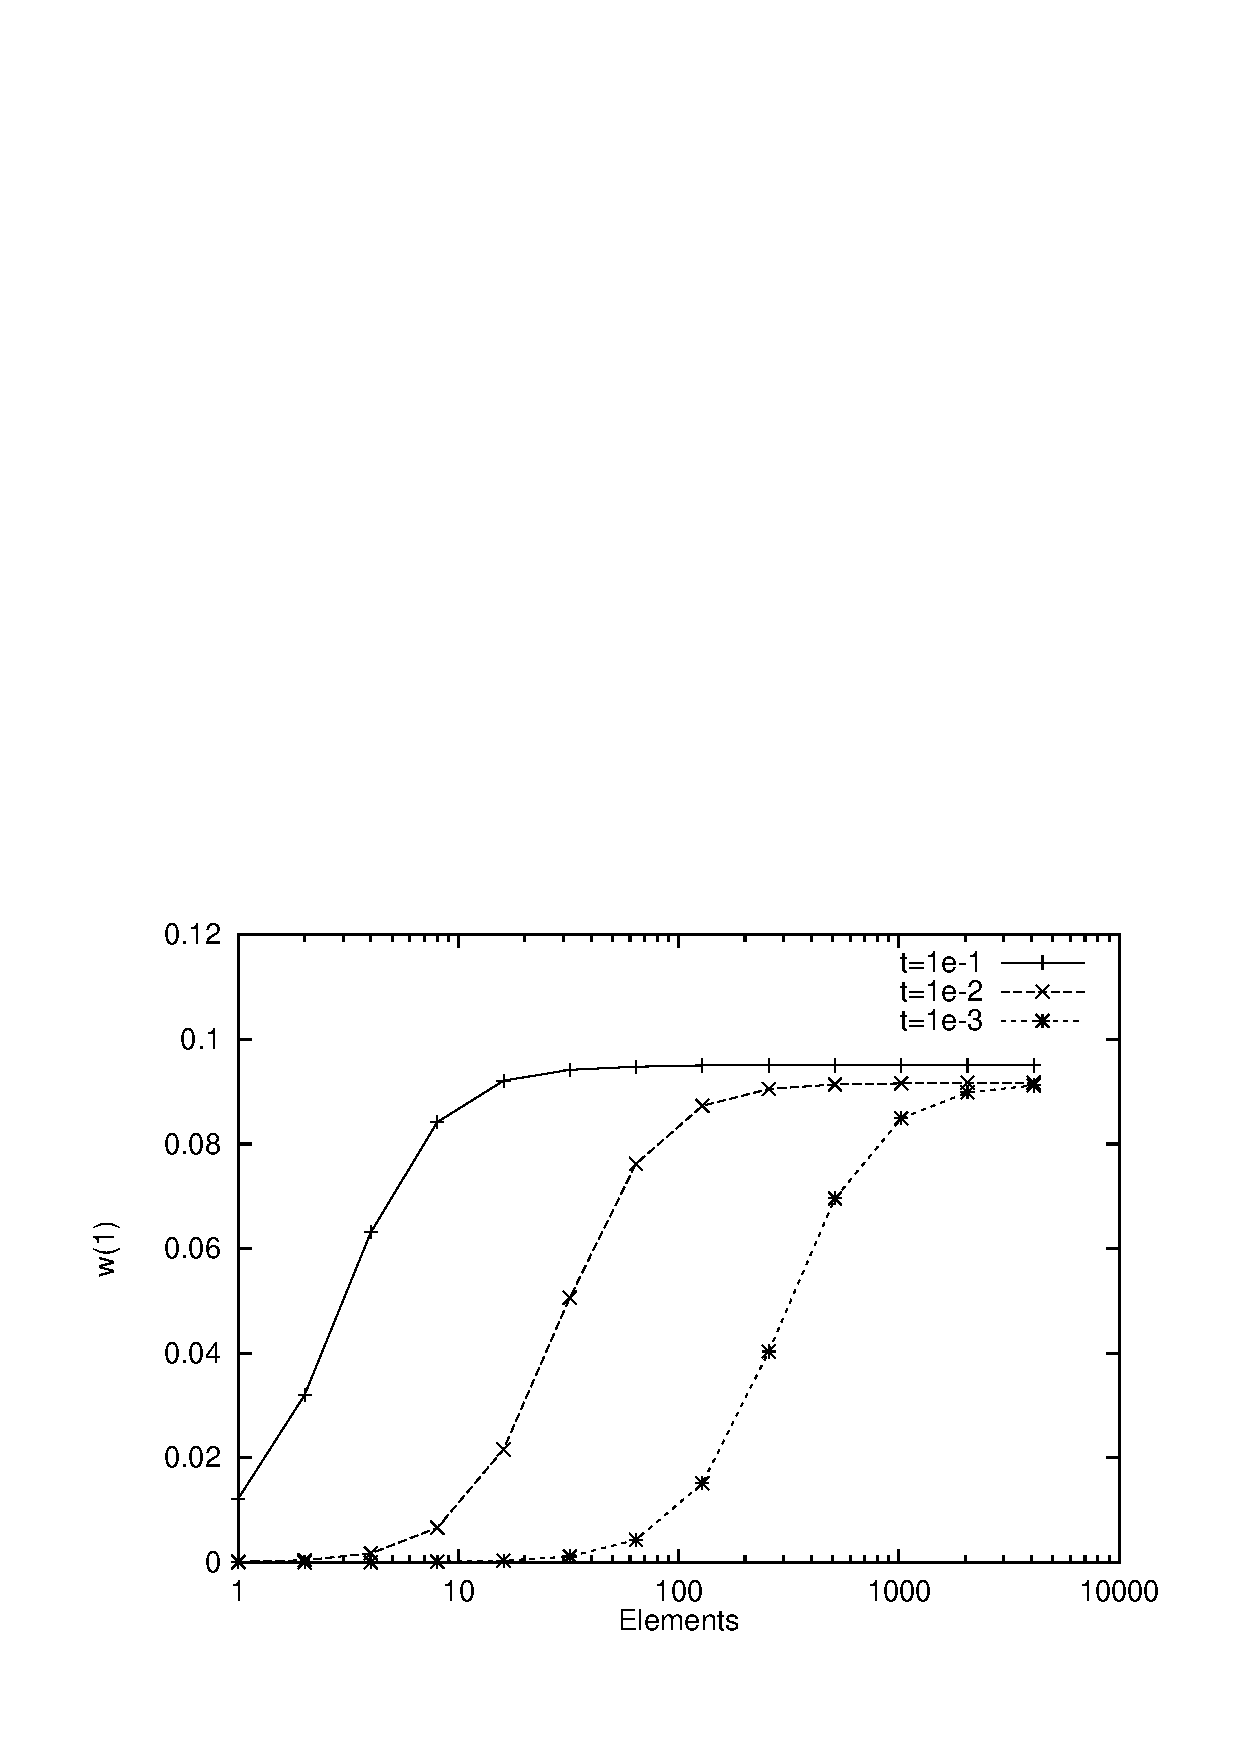
\includegraphics[width=5cm]{pictures/timowntbad}
\hspace{2cm}
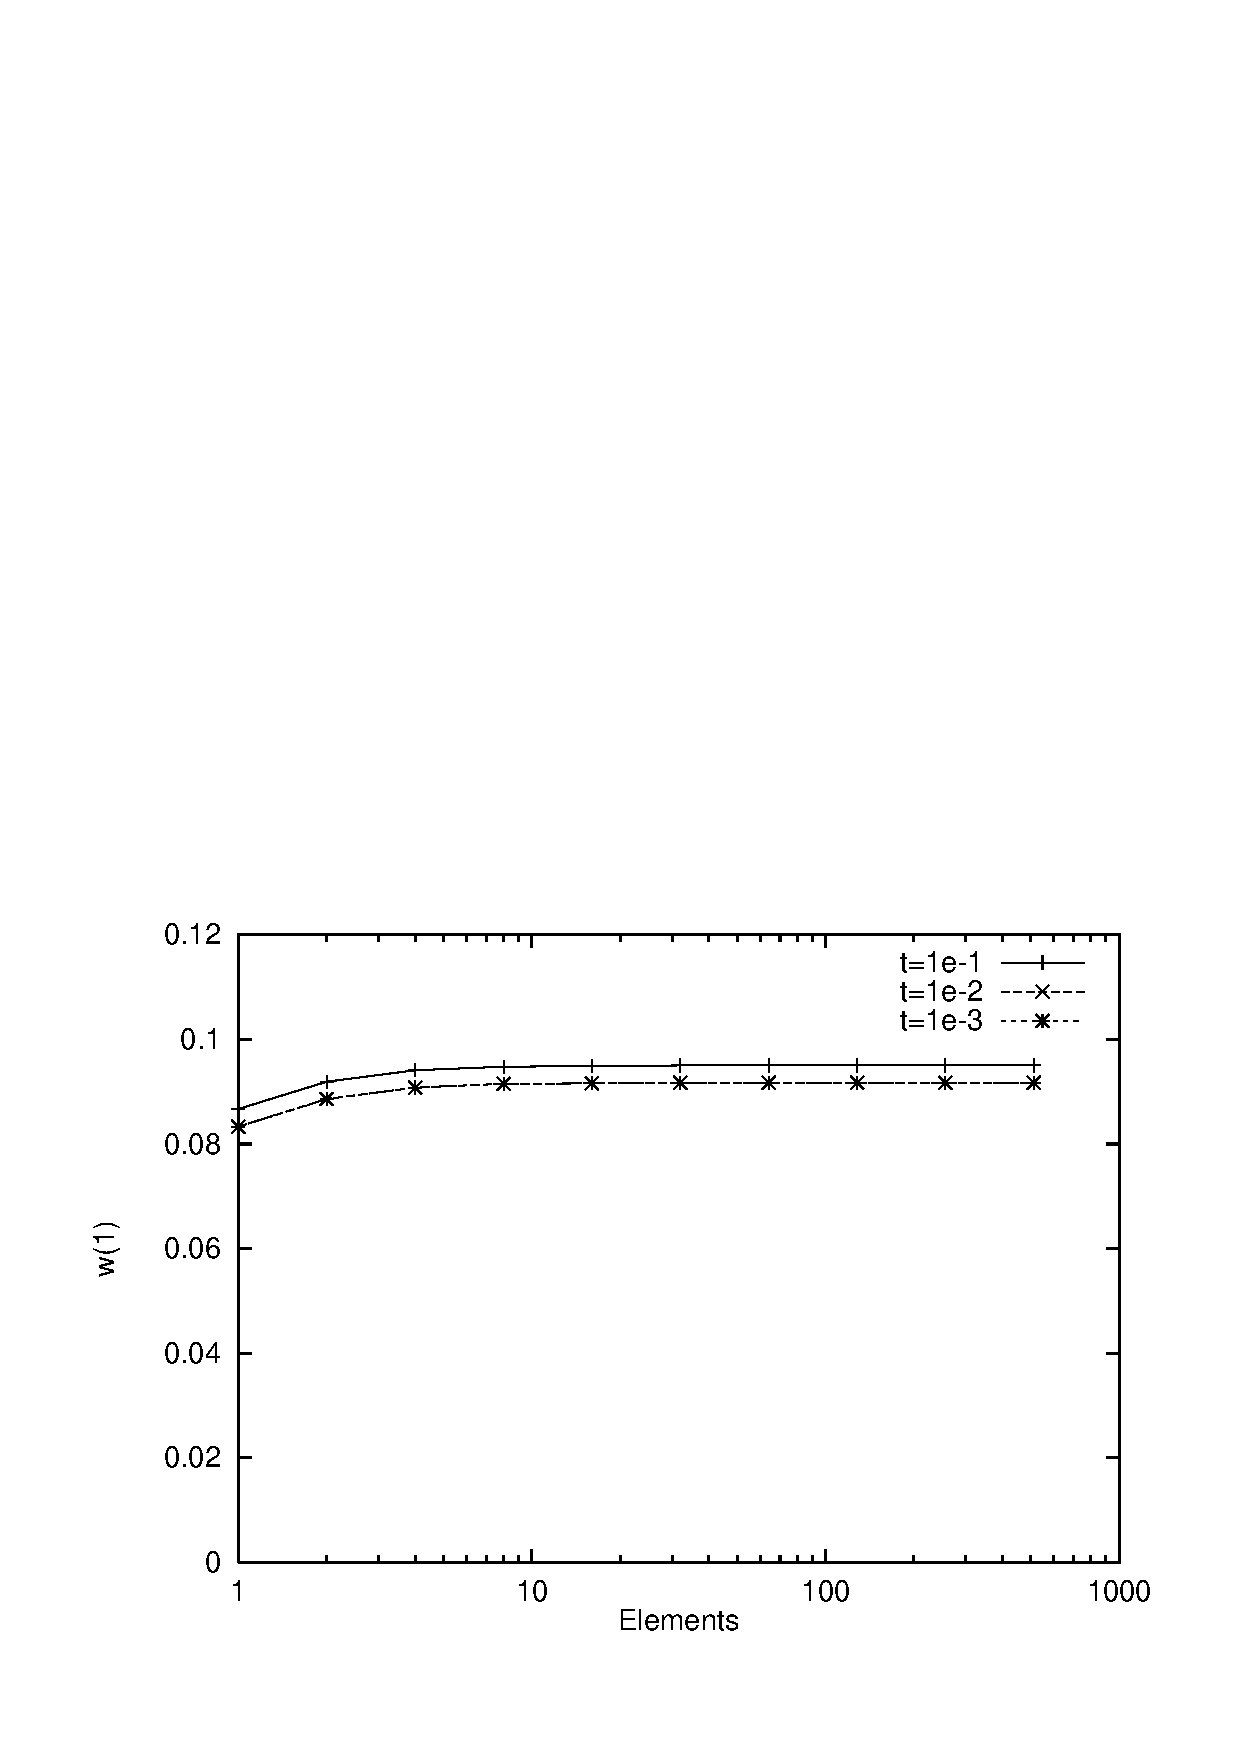
\includegraphics[width=5cm]{pictures/timowntgood}
\end{center}


\section{Maxwell equations}
%
Maxwell equations describe electro-magnetic fields. 
We consider the special case of stationary magnetic fields. 
Maxwell equations are three-dimensional.

A magnetic field is caused by an electric current. We suppose that a current density
$$
j \in [L_2(\Omega)]^3
$$
is given. (Stationary) currents do not have sources, i.e., $\opdiv \, j = 0$. 

The involved (unknown) fields are 
\begin{itemize}
\item
The magnetic flux $B$  (in German: Induktion). The flux is free of sources, i.e.,
$$
\opdiv \, B = 0.
$$
\item 
The magnetic field intensity $H$ (in German: magnetische Feldst\"arke). The field
is related to the current density by Henry's law: 
$$
\int_S j \cdot n \, ds = \int_{\partial S} H \cdot \tau \, ds  \qquad \forall \; \mbox{Surfaces } S
$$
\end{itemize}

By Stokes\'{} Theorem, one can derive Henry's law in differential form:
$$
\opcurl \, H = j
$$
The differential operator is  $\opcurl = \operatorname {rot} = \nabla \times$.
Both fields are related by a material law. The coefficient $\mu$ is called permeability:
$$
B = \mu H
$$

The coefficient $\mu$ is $10^3$ to $10^4$ times larger in iron (and other ferro-magnetic
metals) as in most other media (air). In a larger range, the function $B(H)$ is also highly
non-linear.

Collecting the equations we have
\begin{equation}
\label{equ_bhsystem}
\opdiv \, B = 0 \qquad B = \mu H \qquad \opcurl \, H = j
\end{equation}
In principle, Maxwell equations are valid in the whole $\setR^3$. For simulation, we have
to truncate the domain and have to introduce  artificial boundary conditions.

The picture below shows the magnetic field caused by a tangential current density in
a coil:
\begin{center}
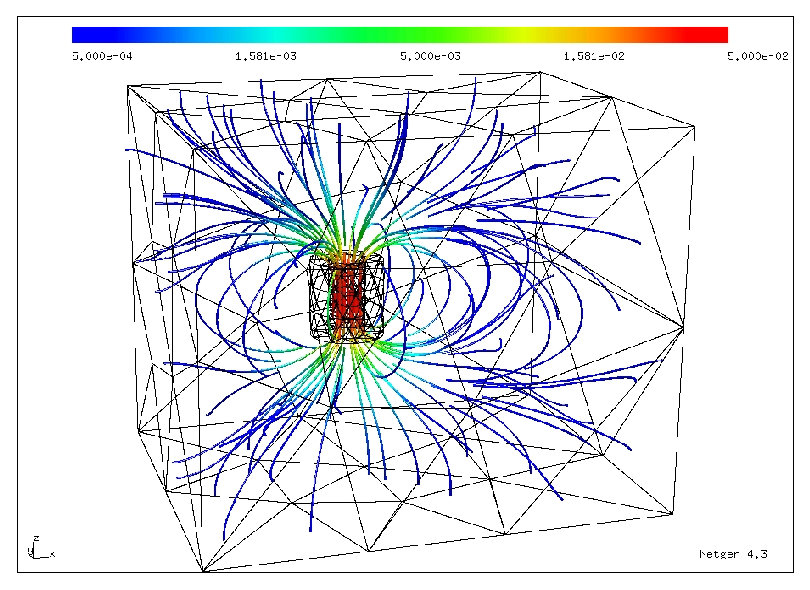
\includegraphics[width=10cm]{pictures/d7_fieldlines}
\end{center}


Compare these equations to the diffusion equation $-\opdiv \, a \nabla u = f$. Here,
we could introduce new unknowns $g = \nabla u$ and $\sigma = a g$. On simply connected
domains, $g$ is a gradient field if and only if $\opcurl g = 0$. We could reformulate
the equations as: Find vector fields $g$ and $\sigma$ such that
$$
\opcurl \, g = 0 \qquad \sigma = a g \qquad \opdiv \, \sigma = -f.
$$

The system of magnetostatic equations looks similar. Only, the right hand side data is
applied to the $\opcurl$-equation, instead of the $\opdiv$-equation. In a similar way as
$\opcurl \, g = 0$ allows to introduce a scalar field $u$ such that $g = \nabla u$,
$\opdiv \, B = 0$ allows to introduce a vector potential $A$ such that
$$
B = \opcurl \, A.
$$
Inserting the vector-potential into the equations (\ref{equ_bhsystem}), one obtains
the second order equation
\begin{equation}
\label{equ_vecpotstrong}
\opcurl \, \mu^{-1}  \opcurl A = j.
\end{equation}

The two original fields $B$ and $H$ can be obtained from the vector potential $A$.

The vector-potential $A$ is not uniquely defined by (\ref{equ_vecpotstrong}). One
may add a gradient field to $A$, and the equation is still true. To obtain a unique
solution, the so called Coloumb-Gauging can be applied:
\begin{equation}
\label{equ_divastrong}
\opdiv \, A = 0.
\end{equation}

As usual, we go over to the weak form. Equations (\ref{equ_vecpotstrong}) and
(\ref{equ_divastrong}) together become: Find $A$ such that
$$
\int_\Omega \mu^{-1} \opcurl A \, \opcurl v \, dx = \int_\Omega j \cdot v \, dx \qquad \forall \, v \in ?
$$
and
$$
\int_\Omega A \cdot \nabla \psi \, dx = 0.
$$

We want to choose the same space for $A$ and the according test functions $v$. But,
then we have more equations than unknowns. The system is still solvable, since we
have made the assumption $\opdiv \, j = 0$, and thus $j$ is in the range of the $\opcurl$-
operator. To obtain a symmetric system, we add a new scalar variable $\varphi$.
The problem is now: Find $A \in V = ?$ and $\varphi \in Q = H^1 / \setR$ such that
\begin{equation} \label{equ_vecpotmixed}
\begin{array}{ccccll}
\int \mu^{-1} \opcurl A \, \cdot \opcurl v \, dx & + & 
\int \nabla \varphi \cdot v \, dx & = & 
\int j \cdot v \, dx \qquad & \forall \, v \in V \\[0.5em]
\int A \cdot \nabla \psi \, dx & & & = & 0 & \forall \, \psi \in Q
\end{array}
\end{equation}

The proper space $V$ is the $H(\opcurl)$: 
$$
H(\opcurl) = \{ v \in [L_2(\Omega)]^3 : \opcurl \, v  \in [L_2(\Omega)]^3 \}
$$
Again, the differential operator $\opcurl$ is understood in the weak sense.
The canonical norm is
$$
\| v \|_{H(\opcurl)} = \left\{ \| v \|_{L_2}^2 + \| \opcurl \, v \|_{L_2}^2 \right\}^{1/2}.
$$

Similar to $H^1$ and $H(\opdiv)$, there exists a trace operator for $H(\opcurl)$. Now,
only the tangential components of the boundary values are well defined:

\begin{theorem} [Trace theorem] There exists a tangential trace operator $\optr_\tau v : H(\opcurl) \rightarrow W(\partial \Omega)$ such that
$$
\optr_\tau v = (v|_{\partial \Omega})_\tau
$$
for smooth functions $v \in [C(\overline \Omega)]^3$. 
\end{theorem}

\begin{theorem} Let $\Omega = \cup \Omega_i$. Assume that $u|_{\Omega_i} \in H(\opcurl,\Omega_i)$,
and the tangential traces are continuous across the interfaces $\gamma_{ij}$. Then $u \in H(\opcurl, \Omega)$.
\end{theorem}


The theorems are according to the ones we have proven for $H(\opdiv)$. But, the proofs (in $\setR^3$) are more involved.

\bigskip

The gradient operator $\nabla$ relates the space $H^1$ and $H(\opcurl)$:
$$
\nabla : H^1 \rightarrow H(\opcurl)
$$

Furthermore, the kernel space
$$
H^0(\opcurl) = \{ v \in H(\opcurl) : \opcurl \, v = 0 \}
$$
is exactly the range of the gradient:
$$
H^0(\opcurl) = \nabla \, H^1
$$



\begin{theorem} The mixed system (\ref{equ_vecpotmixed}) is a well posed problem
on $H(\opcurl) \times H^1/\setR$.
\end{theorem}
{\em Proof:} The bilinear-forms
$$
a(A,v) = \int \mu^{-1} \opcurl A \cdot \opcurl v \, dx
$$
and 
$$
b(v, \varphi) = \int v \cdot \nabla \varphi \, dx
$$
are continuous w.r.t. the norms of $V = H(\opcurl)$ and $Q = H^1/\setR$. 

The LBB-condition in this case is trivial. Choose $v = \nabla \varphi$:
$$
\sup_{v \in H(\opcurl)} \frac{ \int v \nabla \varphi \, dx } { \| v \|_{H(\opcurl)}}
\geq \frac{ \int \nabla \varphi \cdot \nabla \varphi \, dx } { \| \nabla \varphi \|_{H(\opcurl)}}
= \frac{ \| \nabla \varphi \|_{L_2}^2 } { \| \nabla \varphi \|_{L_2}} = \| \nabla \varphi \|_{L_2} \eqc \| \varphi \|_Q
$$

The difficult part is the kernel coercivity of $a(.,.)$. 
The norm involves also the $L_2$-norm, while the bilinear-form only involves the semi-norm
$\| \opcurl \, v \|_{L_2}$. Coercivity cannot hold on the whole $V$: Take a gradient function
$\nabla \psi$. On the kernel, the $L_2$-norm is bounded by the semi-norm:
$$
\| v \|_{L_2} \leqc \| \opcurl \, v \| \qquad \forall \, v \in V_0,
$$
where
$$
V_0 = \{ v \in H(\opcurl) :  \int v \nabla \varphi \, dx = 0 \; \; \forall \, \varphi \in H^1 \}
$$
This is a Friedrichs-like inequality.


\subsubsection{Finite elements in $H(\opcurl)$}
%
We construct finite elements in three dimensions.
The trace theorem implies that functions in $H(\opcurl)$ have continuous tangential 
components across element boundaries (=faces). 

\bigskip

We design tetrahedral finite elements.
The pragmatic approach is to choose the element space as $V_T = P^1$, and choose the 
degrees of freedom as the 
tangential component along the edges in the end-points of the edges. The dimension of
the space is $3 \times \mbox{dim} \{ P^1 \} = 3 \times 4 = 12$, the degrees of freedom
are 2 per edge, i.e., $2 \times 6 = 12$. They are also linearly independent. In each
face, the tangential component has 2 components, and is linear. Thus, the tangential
component has dimension 6. These 6 values are defined by the 6 degrees of freedom of the
3 edges in the face. Neighboring elements share this 6 degrees of freedom in the face,
and thus have the same tangential component.

\bigskip

There is a cheaper element, called N{\'e}d{\'e}lec, or edge-element. 
It has the same accuracy for the $\opcurl$-part (the $B$-field)  as the $P^1$-element. 
It is similar to the Raviart-Thomas element. It contains all constants, 
and some linear polynomials. All 3 components are defined in common. The element space is
$$
V_T = \{ a + b \times x : a, b \in \setR^3 \}.
$$
These are 6 coefficients. For each of the 6 edges of a tetrahedron, one chooses the
integral of the tangential component along the edge
$$
\psi_{E_i}(u) = \int_{E_i} u \cdot \tau_{E_i} \, ds.
$$
\begin{lemma} The basis function $\varphi_{E_i}$ associated with the edge $E_i$ is
$$
\varphi_{E_i} = \lambda_{E_i^1} \nabla \lambda_{E_i^2} - \nabla \lambda_{E_i^2} \lambda_{E_i^1},
$$
where $E_i^1$ and $E_i^2$ are the two vertex numbers of the edge, and $\lambda_1, \ldots \lambda_4$
are the vertex shape functions.
\end{lemma}
{\em Proof: } \begin{itemize}
\item These functions are in $V_T$
\item If $i \neq j$, then $\psi_{E_j}(\varphi_{E_i}) = 0$.
\item $\psi_{E_i}(\varphi_{E_i}) = 1$
\end{itemize}

Thus, edge elements belong to $H(\opcurl)$. Next, we will see that they have also very
interesting properties.

\subsubsection{The de'Rham complex}

The spaces $H^1$, $H(\opcurl)$, $H(\opdiv)$, and $L_2$ form a sequence:

$$
\begin{array}{ccccccc}
H^1             &      \stackrel{\nabla}{\longrightarrow}          &
H(\opcurl)      &      \stackrel{\opcurl}{\longrightarrow}   &
H(\opdiv)       &      \stackrel{\opdiv}{\longrightarrow}    & 
L^2                                                                                    
\end{array}
$$

Since $\nabla H^1 \subset [L_2]^3$, and $\opcurl \nabla = 0$, the gradients 
of $H^1$ functions belong to $H(\opcurl)$. 
Similar, since $\opcurl H(\opcurl) \subset [L_2]^3$, and $\opdiv \opcurl = 0$, 
the $\opcurl$s of $H(\opcurl)$ functions belong to $H(\opdiv)$.

The sequence is a {\em complete} sequence. This means that the kernel of the right
differential operator is exactly the range of the left one (on simply connected domains). 
We have used this property
already in the analysis of the mixed system.

The same property holds on the discrete level: Let \\
\begin{center}
\begin{tabular}{cl}
$W_h$ & be the nodal finite element sub-space  of $H^1$ \\
$V_h$ & be the N\'ed\'elec (edge) finite element sub-space of $H(\opcurl)$ \\
$Q_h$ & be the Raviart-Thomas (face) finite element sub-space of $H(\opdiv)$ \\
$S_h$ & be the piece-wise constant finite element sub-space of $L_2$
\end{tabular}
\end{center}

\begin{theorem}
The finite element spaces form a complete sequence
$$
\begin{array}{ccccccc}
W_h             &      \stackrel{\nabla}{\longrightarrow}          &
V_h             &      \stackrel{\opcurl}{\longrightarrow}   &
Q_h             &      \stackrel{\opdiv}{\longrightarrow}    & 
S_h                                                                                    
\end{array}
$$
\end{theorem}


Now, we discretize the mixed formulation (\ref{equ_vecpotmixed}) by choosing
edge-finite elements for $H(\opcurl)$, and nodal finite elements for $H^1$: Find
$A_h \in V_h$ and $\varphi_h \in W_h$ such that
\begin{equation} \label{equ_vecpotmixedh}
\begin{array}{ccccll}
\int \mu^{-1} \opcurl A_h \, \cdot \opcurl v_h \, dx & + & 
\int \nabla \varphi_h \cdot v_h \, dx & = & 
\int j \cdot v_h \, dx \qquad & \forall \, v_h \in V_h \\[0.5em]
\int A_h \cdot \nabla \psi_h \, dx & & & = & 0 & \forall \, \psi_h \in W_h
\end{array}
\end{equation}
The stability follows (roughly) from the discrete sequence property. The verification
of the LBB condition is the same as on the continuous level. The kernel of the $a(.,.)$-
form are the discrete gradients, the kernel of the $b(.,.)$-form is orthogonal to
the gradients. This implies solvability. The discrete kernel-coercivity (with $h$-independent
constants) is true (nontrivial).


\bigskip


The complete sequences on the continuous level and on the discrete level are connected
in the de'Rham complex: Choose the canonical interpolation operators 
(vertex-interpolation $I^W$, edge-interpolation $I^V$, face-interpolation $I^Q$, 
$L_2$-projection $I^S$). This relates the continuous level to the discrete level:

\begin{equation}
\begin{array}{ccccccc}
H^1             &      \stackrel{\nabla}{\longrightarrow}          &
H(\opcurl)      &      \stackrel{\opcurl}{\longrightarrow}   &
H(\opdiv)       &      \stackrel{\opdiv}{\longrightarrow}    & 
L^2                                                                                    \\[8pt]
\Big\downarrow  \vcenter{ \rlap{$I^W$}}  &                  &
\Big\downarrow  \vcenter{ \rlap{$I^V$}}  &                  &
\Big\downarrow  \vcenter{ \rlap{$I^Q$}}  &                  &
\Big\downarrow  \vcenter{ \rlap{$I^S$}}                             \\[8pt]
 W_h                   &      
\stackrel{\nabla}{\longrightarrow}          &
 V_h       &     
 \stackrel{\opcurl}{\longrightarrow}   &
 Q_h          &      
\stackrel{\opdiv}{\longrightarrow}    & 
S_h  \:.                                                                               \\[8pt]
\end{array}
\label{equ_derham}
\end{equation}

\begin{theorem}
The diagram (\ref{equ_derham}) {\em commutes}:
$$
I^V \nabla = \nabla I^W \qquad
I^Q \opcurl = \opcurl I^V \qquad
I^S \opdiv = \opdiv I^Q
$$
\end{theorem}
{\em Proof:} We prove the first part. Note that the ranges of both,
$\nabla I^W$ and $I^V \nabla$, are in $V_h$. Two functions in $V_h$ coincide if
and only if all functionals coincide. It remains to prove that
$$
\int_E (\nabla I^W w) \cdot \tau \, ds = \int_E (I^V \nabla w)\cdot \tau \, ds
$$
Per definition of the interpolation operator $I^V$ there holds
$$
\int_E (I^V \nabla w)\cdot \tau \, ds = \int_E \nabla w \cdot \tau \, ds
$$
Integrating the tangential derivative gives the difference
$$
\int_E \nabla w \cdot \tau \, ds = \int_E \frac{\partial w}{\partial \tau} \, ds = w(E^2) - w(E^1)
$$
Starting with the left term, and using the property of the nodal interpolation operator,
we obtain
$$
\int_E (\nabla I^W w) \cdot \tau \, ds = (I^W w)(E^2) - (I^W w)(E^1) = w(E^2) - w(E^1).
$$
We have already proven the commutativity of the $H(\opdiv)-L_2$ part of the diagram.
The middle one involves Stokes\'{} theorem.
\hfill $\Box$


This is the key for interpolation error estimates. E.g., in $H(\opcurl)$ there holds
\begin{eqnarray*}
\| u - I^V u \|_{H(\opcurl)}^2 
& = & \| u - I^V u \|_{L_2}^2 + \| \opcurl (I-I^V) u \|_{L_2}^2 \\
& = & \| u - I^V u \|_{L_2}^2 + \| (I-I^Q) \opcurl u \|_{L_2}^2 \\
& \leqc & h^2 \, \| u \|_{H^1}^2 + h^2 \| \opcurl u \|_{H^1}^2 
\end{eqnarray*}
Since the estimates for the $L_2$-term and the $\opcurl$-term are separate, one can
also scale each of them by an arbitrary coefficient.

\bigskip

The sequence is also compatible with transformations. Let $F : \widehat T \rightarrow T$
be an (element) transformation. Choose
\begin{eqnarray*}
w(F(x)) & = & \hat w(x) \\
v(F(x)) & = & (F^\prime)^{-T} \hat v(x) \qquad \qquad \quad \, \mbox{(covariant transformation)}\\
q(F(x)) & = & (\opdet{F^\prime})^{-1} (F^\prime) q(x) \qquad \mbox{(Piola-transformation)} \\
s(F(x)) & = & (\opdet{F^\prime})^{-1} \hat s(x)
\end{eqnarray*}
Then 
\begin{eqnarray*}
\hat v = \nabla \hat w & \Rightarrow & v = \nabla  \, w \\
\hat q = \opcurl \hat v & \Rightarrow & q = \opcurl \, v \\
\hat s = \opdiv \hat q & \Rightarrow & s = \opdiv \, q
\end{eqnarray*}
Using these transformation rules, the implementation of matrix assembling for 
$H(\opcurl)$-equations is very similar to the assembling for $H^1$ problems
(mapping to reference element).


